% !TEX root = ../mechanics.tex
\chapter{不可压无粘流绕流有限翼展的机翼}
前面介绍了无限翼展的翼型气动特性,这一章主
要介绍有限翼展的机翼的气动特性。
\section{下洗和诱导阻力}
有限翼展的机翼是三维的,所以机翼的气动特性
和翼型的气动特性不同,如下图\ref{fig:span}。
\begin{figure}[!ht]
  \centering 
  % ! TEX root = ./aerodynamics/finite_wing.tex
\tikzset{every picture/.style={line width=0.75pt}} %set default line width to 0.75pt        

\begin{tikzpicture}[x=0.75pt,y=0.75pt,yscale=-1,xscale=1]
%uncomment if require: \path (0,379); %set diagram left start at 0, and has height of 379

%Straight Lines [id:da39727047577203534] 
\draw [line width=1.5]    (60,150) -- (60,230) ;
%Straight Lines [id:da11447013885536217] 
\draw [line width=1.5]    (520,150) -- (520,230) ;
%Straight Lines [id:da1723130381460103] 
\draw [line width=1.5]    (60,150) -- (290,120) ;
%Straight Lines [id:da8684705023837216] 
\draw [line width=1.5]    (290,260) -- (520,230) ;
%Straight Lines [id:da6095913924584648] 
\draw [line width=1.5]    (290,120) -- (520,150) ;
%Straight Lines [id:da8952813053936264] 
\draw [line width=1.5]    (60,230) -- (290,260) ;
%Straight Lines [id:da7569741842644373] 
\draw    (60,280) -- (60,320) ;
%Straight Lines [id:da053098603590512106] 
\draw    (520,280) -- (520,320) ;
%Straight Lines [id:da3779632700211717] 
\draw    (290,300) -- (62,300) ;
\draw [shift={(60,300)}, rotate = 360] [color={rgb, 255:red, 0; green, 0; blue, 0 }  ][line width=0.75]    (10.93,-3.29) .. controls (6.95,-1.4) and (3.31,-0.3) .. (0,0) .. controls (3.31,0.3) and (6.95,1.4) .. (10.93,3.29)   ;
%Straight Lines [id:da20615235094281092] 
\draw    (290,300) -- (518,300) ;
\draw [shift={(520,300)}, rotate = 180] [color={rgb, 255:red, 0; green, 0; blue, 0 }  ][line width=0.75]    (10.93,-3.29) .. controls (6.95,-1.4) and (3.31,-0.3) .. (0,0) .. controls (3.31,0.3) and (6.95,1.4) .. (10.93,3.29)   ;
%Straight Lines [id:da791640112777152] 
\draw    (290,190) -- (290,258) ;
\draw [shift={(290,260)}, rotate = 270] [color={rgb, 255:red, 0; green, 0; blue, 0 }  ][line width=0.75]    (10.93,-3.29) .. controls (6.95,-1.4) and (3.31,-0.3) .. (0,0) .. controls (3.31,0.3) and (6.95,1.4) .. (10.93,3.29)   ;
%Straight Lines [id:da325406846820093] 
\draw    (290,190) -- (290,122) ;
\draw [shift={(290,120)}, rotate = 90] [color={rgb, 255:red, 0; green, 0; blue, 0 }  ][line width=0.75]    (10.93,-3.29) .. controls (6.95,-1.4) and (3.31,-0.3) .. (0,0) .. controls (3.31,0.3) and (6.95,1.4) .. (10.93,3.29)   ;
%Straight Lines [id:da8596149068704069] 
\draw    (210,130) -- (210,250) ;
%Straight Lines [id:da41281193810683314] 
\draw    (540,150) -- (580,150) ;
%Straight Lines [id:da047103836611672945] 
\draw    (540,230) -- (580,230) ;
%Straight Lines [id:da16724290585118085] 
\draw    (560,190) -- (560,228) ;
\draw [shift={(560,230)}, rotate = 270] [color={rgb, 255:red, 0; green, 0; blue, 0 }  ][line width=0.75]    (10.93,-3.29) .. controls (6.95,-1.4) and (3.31,-0.3) .. (0,0) .. controls (3.31,0.3) and (6.95,1.4) .. (10.93,3.29)   ;
%Straight Lines [id:da35748881145221234] 
\draw    (560,190) -- (560,152) ;
\draw [shift={(560,150)}, rotate = 90] [color={rgb, 255:red, 0; green, 0; blue, 0 }  ][line width=0.75]    (10.93,-3.29) .. controls (6.95,-1.4) and (3.31,-0.3) .. (0,0) .. controls (3.31,0.3) and (6.95,1.4) .. (10.93,3.29)   ;
%Straight Lines [id:da7041026114003535] 
\draw    (290,30) -- (290,98) ;
\draw [shift={(290,100)}, rotate = 270] [color={rgb, 255:red, 0; green, 0; blue, 0 }  ][line width=0.75]    (10.93,-3.29) .. controls (6.95,-1.4) and (3.31,-0.3) .. (0,0) .. controls (3.31,0.3) and (6.95,1.4) .. (10.93,3.29)   ;
%Curve Lines [id:da3986433821781994] 
\draw    (130,40) .. controls (134.84,120.2) and (130.9,216.64) .. (189.12,269.21) ;
\draw [shift={(190,270)}, rotate = 221.54] [color={rgb, 255:red, 0; green, 0; blue, 0 }  ][line width=0.75]    (10.93,-3.29) .. controls (6.95,-1.4) and (3.31,-0.3) .. (0,0) .. controls (3.31,0.3) and (6.95,1.4) .. (10.93,3.29)   ;
%Curve Lines [id:da7469912525973164] 
\draw  [dash pattern={on 4.5pt off 4.5pt}]  (160,40) .. controls (163.83,129.7) and (157,242.33) .. (111.39,269.21) ;
\draw [shift={(110,270)}, rotate = 331.55] [color={rgb, 255:red, 0; green, 0; blue, 0 }  ][line width=0.75]    (10.93,-3.29) .. controls (6.95,-1.4) and (3.31,-0.3) .. (0,0) .. controls (3.31,0.3) and (6.95,1.4) .. (10.93,3.29)   ;

% Text Node
\draw (409,169) node [anchor=north west][inner sep=0.75pt]   [align=left] {机翼面积$\displaystyle S$};
% Text Node
\draw (298,187) node [anchor=north west][inner sep=0.75pt]   [align=left] {$\displaystyle C_{r}$};
% Text Node
\draw (529,169) node [anchor=north west][inner sep=0.75pt]   [align=left] {翼\\尖};
% Text Node
\draw (259,167) node [anchor=north west][inner sep=0.75pt]   [align=left] {翼\\根};
% Text Node
\draw (179,149) node [anchor=north west][inner sep=0.75pt]   [align=left] {平\\均\\弦\\长};
% Text Node
\draw (255,268) node [anchor=north west][inner sep=0.75pt]   [align=left] {翼展};
% Text Node
\draw (269,309) node [anchor=north west][inner sep=0.75pt]    {$b$};
% Text Node
\draw (569,177) node [anchor=north west][inner sep=0.75pt]    {$C_{t}$};
% Text Node
\draw (299,49) node [anchor=north west][inner sep=0.75pt]   [align=left] {自由来流$\displaystyle V_{\infty }$};


\end{tikzpicture}

  \caption{机翼}
  \label{fig:span}
\end{figure}
在上图中,实线代表机翼上方气流的流动情况;
虚线代表机翼下方气流的流动情况。

下面先介绍几个概念。{\bfseries 翼展(span)}$b$
是机翼两个翼尖之间的距离。{\bfseries 平均弦
长}$c$即机翼的平均气动弦长。对于矩形机翼来说,
机翼的弦长都相等,所以平均气动弦长也等于翼型
的弦长。{\bfseries 后掠角}$\chi$机翼前缘和机身纵轴
的夹角。{\bfseries 根稍比}$\eta$机翼根部的弦长和翼
尖的弦长的比值,$\eta=\frac{c_r}{c_t}$。{\bfseries 
展弦比}$\lambda$,机翼翼展和平均气动弦长的比值。
机翼的面积$S=bc$,即平均气动弦长和翼展乘积。所以
展弦比也等于$\lambda=\frac{b^2}{S}$。

暂时,可以将机翼产生升力的原因归结于机翼下表面的
压强比上表面的大,所以机翼受到一个向上的压强力,
即升力。在翼尖处,由于机翼下表面的压强大于上表面,
所以气流就会这压强的推动下,向上流动,这就是为什么
下表面的气流会向翼尖处流动,而上表面的气流会向翼根
处流动。
\begin{note}
升力产生的原因不全是压强差的问题,还有牛顿第三定律的缘故。
关于压强差产生的原因,不能完全用伯努利方程解释,但确实机翼
上表面的流速大于下表面的流速,参考上一章讨论翼型的升力。
\end{note}
翼尖处气流向上流动,形成了一个涡,这个涡叫做
{\bfseries 翼尖涡(wing-tip vortice)},也叫
{\bfseries 尾涡(trailing vortex)}。
\begin{note}
对于一些大飞机,比如Boeing 747,它们产生的翼尖涡非常
强大,会使得跟得太近的小飞机失控,从而导致事故。
\end{note}
这些翼尖涡会诱导一个小的向下的速度,也就是下洗,用
符号$w$表示。相应地,下洗的速度$w$和自由来流的速度$V_\infty$
的合速度就是流过机翼翼型的实际速度。

自由来流和翼型弦线的夹角叫做攻角,这里我们记为{\bfseries 几何攻角
(geometric angle of attack)}
$\alpha$,如图\ref{fig:effective_attack}
\begin{figure}[!ht]
  \centering
  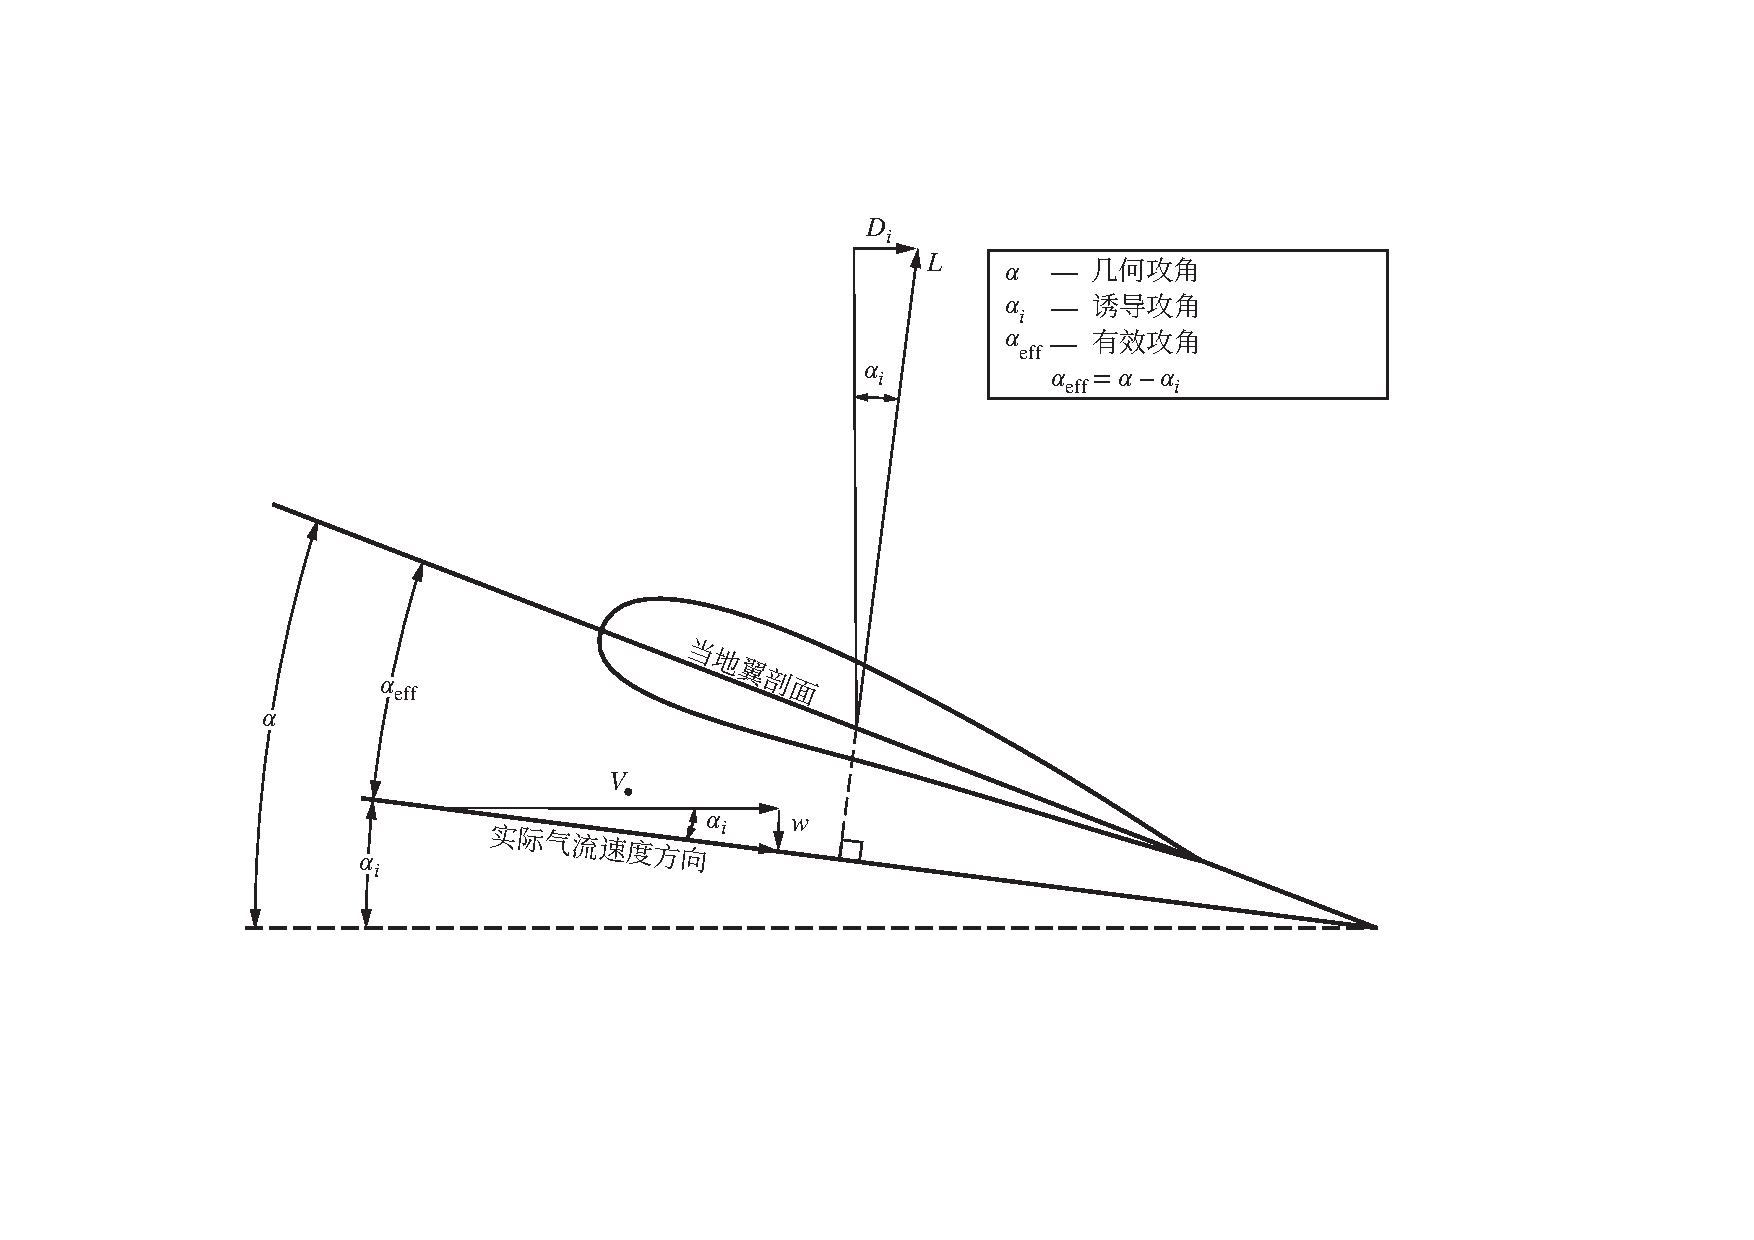
\includegraphics[height=10cm]{./aerodynamics/effective_attack.pdf}
  \caption{下洗对有限翼展机翼当地翼型截面的影响}
  \label{fig:effective_attack}
\end{figure}
当地气流的方向相对于自由来流的方向向下倾斜了$\alpha_i$角度,这个角度
叫做{\bfseries 诱导攻角(induced angle of attack)}。下洗流的存在,
使得当地气流方向向下倾斜,同时对当地翼有剖面主要有两个
影响,如下:
\begin{enumerate}
  \item 实际的迎角是当地气流的方向和当地翼型弦线的夹角,这个夹角
    叫做{\bfseries 有效迎角(effective angle of attack)},记作
    $\alpha_{\mathrm{eff}}$。因此,即使机翼有着几何攻角$\alpha$,当地翼型的
    迎角实际上更下一些,即有效迎角。
    \[
      \alpha_{\mathrm{eff}}=\alpha-\alpha_i
    \]
  \item 当地的升力向量垂直于当地气流方向,因此相较于原来的升力向量
    (竖直方向)落后了角度$\alpha_i$。结果是在自由来流的方向会有
    一个当地升力向量的分量。也就是说,这个阻力是因为下洗的原因产生
    的。这个阻力就被叫做{\bfseries 诱导阻力(induced drag)},记作
    $D_i$。
\end{enumerate}

升力向后倾斜是诱导阻力产生的一种解释,另外的两个解释如下:
\begin{enumerate}
  \item 翼尖涡诱导出来的速度,使得机翼上在自由来流的方向上压强不平衡
    产生了一个向后的力,这个力就是诱导阻力。在这种情况下,诱导阻力也是
    压差阻力的一种。
  \item 翼尖涡中包含了大量的平移和转动的内能,这部分能量必须来自于某个地方
    。事实上,这部分能量几乎都是由飞机的发动机提供的,而发动机是飞机唯一
    相关的动力来源。由于翼尖涡的能量没有任何用处,因此这种能量基本上
    已经丧失。实际上,发动机提供的进入涡流的额外动力就是发动机克服
    诱导阻力所需的额外动力。
\end{enumerate}

\begin{notice}
关于本章的符号问题

对于单位翼展上的升力,阻力,气动力矩,记作$L'$,$D'$,$M'$。
相应的升力系数,阻力系数,力矩系数,记作$c_l$,$c_d$,$c_m$。
对于三维机翼,比如有限翼展的机翼,升力,阻力,气动力矩
记作$L$,$D$,$M$。相应的升力系数,阻力系数,力矩系数
记作$C_L$,$C_D$,$C_M$。对于亚音速的机翼上阻力是诱导阻力$D_i$,
表面摩擦阻力$D_f$和压差阻力$D_P$的和。后面两个阻是因为粘性产生的,
它们的和叫做型阻。对于任何攻角,有限翼展的机翼的型阻系数都是
一样的。
\[
 c_d=\frac{D_f+D_P}{q_\infty S} 
\]
诱导阻力系数是
\[
  C_{D,i}=\frac{D_i}{q_\infty S}
\]
总的阻力系数是
\[
  C_D=c_d+C_{D,i}
\]
\end{notice}

\section{面涡,毕奥--萨伐尔定律和亥姆霍兹定理}
在前面,我们介绍了无限长的直线分布的面涡,实际上,面涡分布
也可以是曲线,沿着涡线积分,就可以得到涡量$\Gamma$,
也是涡强。

考虑涡线上一点的一段有向线段$\mathrm{d}\mathbf{l}$
,在任意一点$P$处,有向线段到该点的径矢是$\mathbf{r}$,
那么有向线段在$P$点处的诱导速度是
\[
  \mathrm{d}\mathbf{V}=\frac{\Gamma}{4 \pi}
  \frac{\mathrm{d}\mathbf{l}\times \mathbf{r}}{\lvert \mathbf{r}\rvert ^3}
\]
这就是毕奥--萨伐尔定律。这和磁场中的毕奥--萨伐尔定律
是一样的。一根无限长的直涡线在任意一点$P$处的诱导速度
是
\[
  V=\frac{\Gamma}{2 \pi h }
\]
其中,$h$是$P$点到涡线的距离。

亥姆霍兹定理的内容如下:
\begin{enumerate}
  \item 面涡的强度沿着它的长度方向是一个常数
  \item 面涡不能在流体中结束,必须在边界上结
    束或者形成一个闭合的路径
\end{enumerate}

下面介绍{\bfseries 升力分布(lift distribution)}的
概念。在给定位置$y_1$升力大小是$L'\left(y_1\right) $,
这个位置处的弦长和迎角分别是$c$和$\alpha$。现在
在另外一个位置$y_2$处的弦长和迎角可能会发生变化,
在这个位置的升力是$L'\left(y_2\right) $ 
\begin{notice}
大部分机翼的翼型的弦长都会随着位置发生变化,矩形
机翼除外;并且每个截面翼型的几何攻角也可能不同,
这是因为机翼有可能发生扭转了。如果翼根处的翼型的
几何攻击大于翼尖的几何攻击,叫做washout ,反之叫
做washin。这种情况叫做{\bfseries 几何扭转(geometrical twist)}。
另外,现代的机翼,不同截面的翼型也不同,所以
每个截面的零升迎角也不同,这叫做{\bfseries 气动扭转(aerodynamic twist)}。
\end{notice}
在不同位置处,单位翼展上的升力是不同的,这就是
机翼上沿着翼展方向上的单位翼展上的升力分布,即$L'=L'(y)$。
根据茹科夫斯基定理,我们知道
\[
  L'=L'(y)=\rho_\infty V_\infty \Gamma(y)
\]
在翼尖处,由于上下表面的压强平衡,所以在翼尖位置,即$y=-\frac{b}{2 }$和
$y= \frac{b}{2}$处的升力等于0 。

总的来说,本章的问题就是计算诱导阻力,总升力,
有限翼展机翼的升力分布。

\section{普朗特经典升力线理论}
普朗特认为,一个强度为$\Gamma$的面涡将被以
某种方式固定在流场中的某个固定位置,这个叫
做
{\bfseries 附着涡(bound vortex)}
,并且产生一个升力
$L'=\rho_\infty V_\infty \Gamma$
。与附着涡相反的是
{\bfseries 自由涡(free vortex)}
,它会随着同一个流体微团运动而遍及全流场。
用一个从
$y=-\frac{b}{2 }$
到
$y=\frac{b}{2 }$
的附着涡替换掉机翼。根据亥姆霍兹定理,涡线
不能再流场中结束,因此假设在翼尖的下游有两
条向无限远方向延伸的自由涡。因为附着涡和自
由涡叠加而形成的涡系形状上像一个马蹄,因此
叫做
{\bfseries 马蹄涡(horseshoe vortex)}。
附着涡不会在翼展这段位置上诱导出下洗的速度
,因此,下洗速度$w $都是由自由涡诱导出来的
。我们可以用毕奥萨伐尔定律计算出翼展上的诱
导速度
\[
  w(y)=-\frac{\Gamma}{4\pi(\frac{b}{2}+y)}
       -\frac{\Gamma}{4\pi(\frac{b}{2}-y)}
       =-\frac{\Gamma}{4\pi}\frac{b}{\left
     (\frac{b}{2}\right)^2-y^2}
\]

单个马蹄涡产生的下洗速度分布和实际情况并不
一致,并且在翼尖处诱导速度将接近无穷大,这
显然不合理。假设在翼展上分布由大量的马蹄涡
形成一个马蹄涡系,每个马蹄涡的附着涡长度都
不一样,并且强度也不一样,但是每条附着涡都
还是沿着一条直线分布的,这条线叫做
{\bfseries 升力线(lifting line)}。
这一部分请参考教材。
请记住尾涡的强度等于升力线上面涡强度的变化
。

如果叠加无穷多的马蹄涡,形成一个马蹄涡系,
这样沿翼展方向,面涡强度
$\Gamma$
就变成了一个连续分布的函数,也就是
$\Gamma=\Gamma(y)$
在微元长度上的面涡强度就是
\[
  \mathrm{d}\Gamma=\left(\frac{\mathrm{d}
  \Gamma}{\mathrm{d}y}\right)
  \mathrm{d}y
\]
相应地,尾涡的强度就等于
$\mathrm{d}\Gamma$
的变化。那么任意一点$y $处的涡强
$\mathrm{d}\Gamma$
在$y_0$ 处的诱导速度就是
\[
  \mathrm{d}w=-\frac{(\mathrm{d}\Gamma 
  / \mathrm{d}y)\mathrm{d}y}{4\pi(y_0-y)}
\]
这个速度是在$y $处的半无限长的自由涡在点
$y_0 $诱导出的下洗速度。这个负号表示速度方
向是向下的。在$y_0 $点的总诱导速度由下式给
出
\[
  w=-\frac{1}{4\pi}
  \int_{-\frac{b}{2}}^{\frac{b}{2 }}
  \frac{\left(\frac{\mathrm{d}\Gamma}{\mathrm{d}y}\right)}
  {y_0-y}\mathrm{d}y
\]
上式很重要,它给出了在$y_0 $处由所有自由涡
诱导出来的下洗速度。

从图\ref{fig:effective_attack}中,我们得到
诱导迎角的大小
\[
  \alpha_i(y_0)=\tan ^{-1}
  \left(\frac{-w(y_0) }{V_\infty}\right)
\]
一般来说,$w $远小于$V_\infty$,所以诱导迎
角也可以写成
\[
  \alpha_i(y_0)= -\frac{w(y_0) }{V_\infty}
\]
再将前面计算下洗速度的积分公式代入就可以得
到
\begin{empheq}[box=\widefbox]{equation*}
  \alpha_i(y_0)=\frac{1}{4\pi V_\infty}
  \int_{-\frac{b}{2 }}^{\frac{b}{2 }}
  \frac{\left(\frac{\mathrm{d}\Gamma}{\mathrm{d}y}\right) }
  {y_0-y}\mathrm{d}y
\end{empheq}
这样我们就可以通过涡强分布来计算诱导迎角的
大小。

根据前面所述的几何迎角和有效迎角之间的关系
,我们可以计算处有效迎角
\[
  \alpha_{\mathrm{eff}}= \alpha-\alpha_i
  =\alpha-\frac{1}{4\pi V_\infty}
  \int_{-\frac{b}{2 }}^{\frac{b}{2 }}
  \frac{\left(\frac{\mathrm{d}\Gamma}{\mathrm{d}y}\right) }
  {y_0-y}\mathrm{d}y
\]
然后根据前面我们讨论的翼型的升力曲线,我们
就可以得到在$y_0 $处的升力系数
\[
  c_l=a_0\left(\alpha_{\mathrm{eff}}(y_0)-\alpha_{L=0}\right)
  =2\pi\left(\alpha_{\mathrm{eff}}(y_0)-\alpha_{L=0}\right)
\]
在任何情况下,零升迎角都是已知的,它只与翼
型有关。同样,升力不仅可以通过升力系数进行
计算,还可以用茹科夫斯基升力公式进行计算,
也就是
\[
  L'=\frac{1}{2}\rho_\infty V_\infty ^2 
  c(y_0)c_l
  = \rho_\infty V_\infty \Gamma\left(y_0\right) 
\]
于是我们又可以得到计算机翼单位翼展上升力系
数的第二个公式,即
\[
  c_l=\frac{2 \Gamma\left(y_0\right) }{V_\infty c(y_0) }
\]
所以有效攻角也可以用下式计算
\[
  \alpha_{\mathrm{eff}}=\frac{\Gamma\left(y_0\right) }
  {\pi V_\infty c\left(y_0\right) }+\alpha_{L=0}
\]
带入到
\[
  \alpha=\alpha_{\mathrm{eff}}+\alpha_i
\]
中,我们就得到了几何攻角的计算公式,即
\begin{empheq}[box=\widefbox]{equation*}
  \alpha(y_0)= 
  \frac{\Gamma(y_0) }{\pi V_\infty c(y_0) }+
  \alpha_{L=0}(y_0)+
  \frac{1}{4\pi V_\infty}
  \int _{-\frac{b}{2}}^{\frac{b}{2 }}
  \frac{\frac{\mathrm{d}\Gamma }{\mathrm{d}y}}
  {y_0-y}\mathrm{d}y
\end{empheq}
这就是普朗特升力线理论的基本方程。这表明了几何
迎角等于有效迎角加上诱导迎角。这个方程是一个积
分---微分方程,唯一的未知量就是$\Gamma $,其他
量都是已知的。

从基本方程得出$\Gamma=\Gamma(y_0)$的解给了我们
三个关于有限翼展机翼的基本性质,即:
\begin{enumerate}
  \item 升力分布可以从库塔--- 茹科夫斯基定理中
    得到,即
    \[
      L'(y_0)=\rho_\infty V_\infty \Gamma(y_0) 
    \]
  \item 总升力可以对第一点性质中的公式积分得到
    ,即
    \[
      L=\int_{-\frac{b}{2 }}^{\frac{b}{2}}L'(y)\mathrm{d}y
    \]
    或
    \[
      L=\rho_\infty V_\infty 
      \int_{-\frac{b}{2 }}^{\frac{b}{2}}\Gamma(y)\mathrm{d}y
    \]
    升力系数可以由下式给出
    \[
      C_L=\frac{L}{q_\infty S}=\frac{2}{V_\infty S}= 
      \int _{-\frac{b}{2}}^{\frac{b}{2}}\Gamma(y)\mathrm{d}y
    \]
  \item 从图\ref{fig:span}中,我们可以得到诱导
    阻力的计算公式,即
    \[
      D' _i=L' _i\sin \alpha_i
    \]
    因为诱导迎角很小,所以
    \[
      D' _i=L' _i\alpha_i
    \] 
    于是总的诱导阻力由下面的积分公式给出
    \[
      D_i=\int _{-\frac{b}{2}}
      ^{\frac{b}{2}}L'(y)\alpha_i(y)
      \mathrm{d}y 
    \]
    或
    \[
      D_i= \rho_\infty V_\infty 
      \int _{-\frac{b}{2}}
      ^{\frac{b}{2}}
      \Gamma(y)\alpha_i(y)\mathrm{d}y
    \]

    相应地,诱导阻力系数就是
    \[
      C_{D,i}=\frac{D_i}{q_\infty S}
      =\frac{2}{V_\infty S}
      \int _{-\frac{b}{2}}
      ^{\frac{b}{2}}
      \Gamma(y)\alpha_i(y)\mathrm{d}y
    \]
\end{enumerate}

在介绍椭圆形升力分布之前,先介绍一个重要的结论,即
{\bfseries 椭圆形机翼的升力分布就是椭圆形升力分布,
椭圆形升力分布的机翼就是椭圆形机翼}。
\subsection{椭圆型升力分布}
考虑一个涡强分布,即
\[
  \Gamma(y)=\Gamma_0
  \sqrt{1-\left(\frac{2y}{b}\right)^2} 
\]
请记住:
\begin{enumerate}
  \item $\Gamma_0$是涡强的初始值,是在
    翼展中间的值
  \item 环量随着坐标$y $椭圆型地变化,
    单位翼展上的升力由下式给出
    \[
      L'(y)=\rho_\infty V_\infty 
      \Gamma_0
      \sqrt{1-\left(\frac{2y}{b }\right)^2} 
    \] 
    \item $\Gamma\left(-\frac{b}{2}\right)= 
      \Gamma\left(\frac{b}{2}\right) $,环量
      和升力在翼尖出等于0 。
\end{enumerate}

首先,我们先计算下洗,
\[
  \frac{\mathrm{d}\Gamma}{\mathrm{d}y}
  =-\frac{4\Gamma_0}{b^2}
  \frac{y}{\left(1-\frac{4y^2}{b^2}\right)^{\frac{1}{2}}}
\]
带入到下式中
\[
  w(y_0)=-\frac{1}{4\pi}
  \int _{-\frac{b}{2}}^{\frac{b}{2}}
  \frac{\mathrm{d}\Gamma / \mathrm{d}y}{y_0-y}\mathrm{d}y
\]
得到
\[
  w(y_0)=\frac{\Gamma_0}{\pi b^2}
  \int _{-\frac{b}{2}}^{\frac{b}{2}}
  \frac{y}{\left(1-\frac{4y^2}{b^2}\right)^{\frac{1}{2}}(y_0-y)}\mathrm{d}y
\]
作变量替换
\[
  y=\frac{b}{2}\cos \theta \qquad \mathrm{d}y=-\frac{b}{2}\sin \theta \mathrm{d}\theta
\]
上述积分就变成了
\[
  w(\theta_0)=-\frac{\Gamma_0}{2 \pi b }
  \int _0 ^\pi \frac{\cos \theta}{\cos \theta-\cos \theta_0}\mathrm{d} \theta
\]
计算得到
\[
  w(\theta_0)=-\frac{\Gamma_0}{2b}
\]
这结果表明,{\color{noteorange}\bfseries 对于椭圆型升力分布的机翼来说,
下洗速度是一个常数}。这个结论很有趣也很重要。
我们可以计算得到诱导迎角
\[
  \alpha_i=-\frac{w }{V_\infty }= \frac{\Gamma_0}{2 b V_\infty}
\]
对于椭圆型分布的机翼来说,诱导迎角也是一个常数。
并且,当翼展趋于无穷大时,诱导迎角和下洗都趋于0 。
这就是前面我们讨论的翼型理论。一个关于诱导迎角
更有用的公式如下:
\[
  L=\rho_\infty V_\infty \Gamma_0 
  \int _{-\frac{b}{2}}^{\frac{b}{2}}
  \left(1-\frac{4y^2}{b^2}\right)^{\frac{1}{2}}
  \mathrm{d}y
\]
再用前面所说的三角代换,计算这个积分得到
\[
  L=\rho_\infty V_\infty \Gamma_0 \frac{b}{4}\pi
\]
于是就得到了$\Gamma_0$的计算公式
\[
  \Gamma_0=\frac{4L}{\rho_\infty V_\infty b \pi}
\]
其中$L=\frac{1}{2}\rho_\infty V_\infty^2 S C_L$
于是
\[
  \Gamma_0=\frac{2V_\infty S C_L}{b \pi}
\]
诱导迎角的计算公式就可以写成
\[
  \alpha_i = \frac{2V_\infty S C_L}{b \pi} 
  \frac{1}{2b V_\infty }
\]
或者
\[
  \alpha _i =\frac{S C_L}{\pi b^2}
\]
机翼的一个重要几何参数就是{\bfseries 展弦比(aspect ratio)},
这里记作AR,即
\[
  \mathrm{AR}=\frac{b^2}{S}
\]
于是,上式就可以写成
\[
  \alpha_i=\frac{C_L}{\pi \mathrm{AR}}
\]
诱导阻力系数有下式给出,请记住诱导迎角是一个
常数
\[
  C_{D,i}=\frac{2\alpha_i}{V_\infty S}
  \int _{-\frac{b}{2}}^{\frac{b}{2}}
  \Gamma(y)\mathrm{d}y
  =\frac{2\alpha_i \Gamma_0}{V_\infty S}
  \frac{b}{2}
  \int _0^\pi \sin^2\theta \mathrm{d}  \theta
  =\frac{\pi \alpha_i \Gamma_0 b }{2 V_\infty S}
\]
代入$\alpha_i=\frac{C_L}{\pi \mathrm{AR}}$得到
\[
  C_{D,i}=\frac{C_L^2}{\pi \mathrm{AR}}
\]
这是一个很重要的结果,它表明诱导阻力系数正比于
升力系数的平方。前面我们已经知道,诱导阻力是翼
尖涡出现的结果,而翼尖涡是由于翼尖处上下表面压
强差的结果。升力也同样是由于上下表面的压强差产
生的。因此,诱导阻力与有限翼展机翼上的升力产生
密切相关。事实上,诱导阻力经常被叫做
{\bfseries 升致阻力(drag due to lift)}。
显然,任何一架飞机不能免费地产生升力,诱导阻力
就是产生升力的代价。飞机克服诱导阻力所需的功率
就是产生升力所需的功率。诱导阻力系数随升力系数
增大而迅速增大,当升力系数比较大的时候,诱导阻
力系数就变成总阻力系数的一个重要组成部分了。
\begin{notice}
比如飞机起飞和着陆时,因为飞机的速度比较小,而
需要比较大的升力,这个时候就需要我们在上一章中
提到的增升装置,当增升装置启用的时候,飞行阻力
也会相应变大很多。
\end{notice}
甚至在一个很高的巡航速度飞行的时候,诱导阻力系
数都占到总阻力系数的25\%。

另外一个重要的结论是
{\color{noteorange} \bfseries 诱导阻力系数反比
于展弦比 }。因此,为了减小阻力,我们希望机翼有
一个尽可能最大的展弦比。但是,展弦比很大,机翼
的结构强度就会相应减小,或者说机翼更难设计。对
于一般的飞行器来说,展弦比是气动设计和结构设计
中的一个两难的选择。

椭圆型升力分布的机翼的一些其他性质如下。考虑一
个没有几何扭转的机翼,同时也没有气动扭转。因为
整个机翼上的诱导迎角是一个常数,所以有效迎角也
是一个常数,因此当地截面翼型的升力系数如下
\[
  c_l=a_0(\alpha_{\mathrm{eff}}-\alpha_{L=0})
\]
假设每个截面翼型的升力系数曲线的斜率都是$a_0$
,都是$2\pi$。因此,沿着翼展方向,升力系数也是
常数,单位翼展上的升力由下式给出
\[
  L'(y)q_\infty c_l
\]
于是,我们就可以求得这个机翼的弦长分布
\[
  c(y)=\frac{L'(y) }{q_\infty c_l}
\]
因为动压和升力系数沿着翼展方向都是常数,所以对
于这样一个椭圆型升力分布的机翼,弦长沿翼展方向
也必须是椭圆型变化的。这种情况下,我们说这个机
翼就是椭圆形机翼,即从上往下看,机翼的形状是椭
圆形的。

\subsection{一般升力分布}
考虑一个积分变换
\[
  y=-\frac{b}{2}
\]
对于任意一个机翼的一般环量分布,我们可以把$\Gamma(y) $
展开成一个傅里叶正弦级数,即
\[
  \Gamma(\theta)=2 b V_\infty 
  \sum_{n=1}^{N} A_n \sin n \theta
\]
于是我们就可以得到
\[
  \frac{\mathrm{d}\Gamma}{\mathrm{d}y}= 
  2 b V_\infty 
  \sum_{n=1}^{N} n \cos n \theta \frac{\mathrm{d} \theta}{\mathrm{d} y}
\]
几何攻角的计算公式如下
\[
  \alpha(\theta_0)= 
  \frac{2b }{\pi c(\theta_0)}
  \sum_{n=1}^{N} A_n \sin n \theta 
  +\alpha_{L=0}(\theta_0)+
  \sum_{n=1}^{N} \frac{\sin n \theta_0}{\theta_0}
\]
给出升力系数计算公式
\[
  C_L=\frac{2b^2}{S}
  \sum_{n=1}^{N} A_n \int _0^\pi 
  \sin n \theta \sin \theta \mathrm{d} \theta
\]
计算上面这个积分得到
\[
  C_L=A_1\pi \mathrm{AR}
\]
诱导阻力系数的计算公式
\[
  C_{D,i}= \frac{2b^2}{S }\int _0^\pi 
  \left(\sum_{n=1}^{N} A_n \sin n \theta \right) 
  \alpha_i(\theta) \sin \theta \mathrm{d} \theta
\]
诱导迎角的计算公式
\[
  \alpha_i (y_0)= \frac{1}{\pi}
  \sum_{n=1}^{N} n A_n \int _0 ^\pi 
  \frac{\cos n \theta}{\cos \theta -\theta_0}\mathrm{d} \theta
\]
于是
\[
  \alpha_i(\theta_0)
  =\sum_{n=1}^{N} n A_n \frac{\sin n \theta_0}{\sin \theta_0}
\]
代入到诱导阻力的计算公式中
\[
  C_{D,i}=\pi \mathrm{AR}A_1^2 
  \left[1+\sum_{n=2}^{N} n\left(\frac{A_n}{A_1}\right)^2\right]
\] 
将升力系数的计算公式代入,并令$\delta = \sum\limits_{n=2}^{N} n (A_n / A_1)^2$
得到
\begin{empheq}[box=\widefbox]{align*}
  C_{D,i}&=\frac{C_L^2}{\pi \mathrm{AR}}(1+\delta)\\
         &= \frac{C_L^2}{\pi e \mathrm{AR}}
\end{empheq}
其中$e=(1+\delta)^{-1}$,并且$e$是一个小于1的系数。
当$\delta=0 $和$e=1$的时候,升力分布是一个椭圆型的升力分布。

\subsection{展弦比的影响}
从诱导阻力系数的计算公式中,可以发现展弦比和诱导阻力系数
是反比关系。因此,最小化诱导阻力的主要设计因素不是让
升力分布更加接近椭圆形而是是展弦比尽可能大。
回忆一下,总阻力系数由下式给出
\[
  C_D=c_d+\frac{C_L^2 }{\pi e \mathrm{AR}}
\]
不难拿得出总阻力系数和升力系数是二次相关的。

翼型和机翼的性质有两个主要的差别。一个是前面讨论的
诱导阻力系数,即机翼会产生诱导阻力;
另外一个是接下来要讨论的升力系数曲线。
定义机翼的升力线斜率是$a=\frac{\mathrm{d}C_L}{\mathrm{d}\alpha}$。
与当地截面翼型的升力线斜率相比,我们知道$a<a_0$。
这是因为诱导迎角的存在,使得有效迎角小于实际迎角。
但是零升迎角却没有发生变化,这就相当于$x$轴被拉长了。
也就是
\[
  \frac{\mathrm{d}C_l}{\mathrm{d}(\alpha-\alpha_i)}=a_0
\]
积分我们得到
\[
  C_L=a_0(\alpha-\frac{C_L}{\pi \mathrm{AR}})+const
\]
整理一下,不难得到
\begin{empheq}[box=\widefbox]{equation*}
  a=\frac{a_0}{1+\frac{a_0}{\pi \mathrm{AR}}}
\end{empheq}
上式只适用于椭圆形机翼,
对于一般升力分布的机翼来说,升力线斜率的计算公式
如下
\[
  a=\frac{a_0}{1+(1+\tau)\frac{a_0}{\pi \mathrm{AR}}}
\]
$\tau$是傅里叶级数系数$A_n$的函数,一般$0.05\leq \tau \geq 0.25$

展弦比越大,机翼的升力线斜率就越接近翼型的升力线斜率。
% ! TEX root = ./finite_wing.tex
\section{总结}
在总结之前,请确保你对一下概念都是熟悉的,
请保证你对一下的内容式舒适的。
\begin{summary}
  \begin{enumerate}
    \item 展弦比\hspace{2em}根稍比\hspace{2em}
      诱导阻力\hspace{2em}下洗\hspace{2em}
      诱导迎角\hspace{2em}有效迎角\hspace{2em}
      几何迎角
    \item 诱导迎角,几何迎角,有效迎角之间的关系
      \[
        \alpha_{\mathrm{eff}}=\alpha-\alpha_i
      \]
    \item 椭圆形机翼的计算公式
      \begin{enumerate}
        \item 下洗
          \[
            w=-\frac{\Gamma_0}{2b}
          \]
          \item 诱导迎角
            \[
              \alpha_i=\frac{C_L}{\pi \mathrm{AR}}
            \]
          \item 诱导阻力系数
            \begin{empheq}[box=\bluebox]{equation*}
              C_{D,i}=\frac{C_L^2 }{\pi \mathrm{AR}}
            \end{empheq}
          \item 升力线斜率
            \begin{empheq}[box=\bluebox]{equation*}
              a=\frac{a_0}{1+\frac{a_0}{\pi \mathrm{AR}}}
            \end{empheq}
      \end{enumerate}
    \item 一般机翼
      \begin{enumerate}
        \item 诱导阻力系数
          \begin{empheq}[box=\bluebox]{equation}
            C_{D,i}=\frac{C_L^2}{\pi \mathrm{AR}}(1+\delta)= 
            \frac{C_L^2}{\pi e \mathrm{AR}}
          \end{empheq}
        \item 升力线斜率
          \begin{empheq}[box=\bluebox]{equation}
            a=\frac{a_0}{1+(1+\tau)\frac{a_0}{\pi \mathrm{AR}}}
          \end{empheq}
      \end{enumerate}
  \end{enumerate}
\end{summary}

